% THIS IS SIGPROC-SP.TEX - VERSION 3.1
% WORKS WITH V3.2SP OF ACM_PROC_ARTICLE-SP.CLS
% APRIL 2009
%
% It is an example file showing how to use the 'acm_proc_article-sp.cls' V3.2SP
% LaTeX2e document class file for Conference Proceedings submissions.
% ----------------------------------------------------------------------------------------------------------------
% This .tex file (and associated .cls V3.2SP) *DOES NOT* produce:
%       1) The Permission Statement
%       2) The Conference (location) Info information
%       3) The Copyright Line with ACM data
%       4) Page numbering
% ---------------------------------------------------------------------------------------------------------------
% It is an example which *does* use the .bib file (from which the .bbl file
% is produced).
% REMEMBER HOWEVER: After having produced the .bbl file,
% and prior to final submission,
% you need to 'insert'  your .bbl file into your source .tex file so as to provide
% ONE 'self-contained' source file.
%
% Questions regarding SIGS should be sent to
% Adrienne Griscti ---> griscti@acm.org
%
% Questions/suggestions regarding the guidelines, .tex and .cls files, etc. to
% Gerald Murray ---> murray@hq.acm.org
%
% For tracking purposes - this is V3.1SP - APRIL 2009

\documentclass{acm_proc_article-sp}
\usepackage{hyperref}
\begin{document}

\title{CS 472 - Project \#4 - Brood Recombination}
\subtitle{University of Idaho - Evolutionary Computation (CS 472)}
%
% You need the command \numberofauthors to handle the 'placement
% and alignment' of the authors beneath the title.
%
% For aesthetic reasons, we recommend 'three authors at a time'
% i.e. three 'name/affiliation blocks' be placed beneath the title.
%
% NOTE: You are NOT restricted in how many 'rows' of
% "name/affiliations" may appear. We just ask that you restrict
% the number of 'columns' to three.
%
% Because of the available 'opening page real-estate'
% we ask you to refrain from putting more than six authors
% (two rows with three columns) beneath the article title.
% More than six makes the first-page appear very cluttered indeed.
%
% Use the \alignauthor commands to handle the names
% and affiliations for an 'aesthetic maximum' of six authors.
% Add names, affiliations, addresses for
% the seventh etc. author(s) as the argument for the
% \additionalauthors command.
% These 'additional authors' will be output/set for you
% without further effort on your part as the last section in
% the body of your article BEFORE References or any Appendices.

\numberofauthors{1} %  in this sample file, there are a *total*
% of EIGHT authors. SIX appear on the 'first-page' (for formatting
% reasons) and the remaining two appear in the \additionalauthors section.
%
\author{
% You can go ahead and credit any number of authors here,
% e.g. one 'row of three' or two rows (consisting of one row of three
% and a second row of one, two or three).
%
% The command \alignauthor (no curly braces needed) should
% precede each author name, affiliation/snail-mail address and
% e-mail address. Additionally, tag each line of
% affiliation/address with \affaddr, and tag the
% e-mail address with \email.
%
% 1st. author
\alignauthor
Andrew Schwartzmeyer\\
       \affaddr{University of Idaho}\\
       \affaddr{709 S Deakin St}\\
       \affaddr{Moscow, ID, USA}\\
       \email{andrew@schwartzmeyer.com}
}
\date{9 May 2014}

\maketitle
\begin{abstract}
For the University of Idaho's Evolutionary Computation (CS 472)
Project \#4 I studied the cost of brood recombination for increasing
performance on the Santa Fe Trail problem. My hypothesis was that
brood recombination's improvement to the crossover process would
compensate for its computational overhead. A genetic program to model
an artifical ant with the goal of eating as much food as possible on
the Santa Fe trail was implemented using C++11. It was extensively
profiled for performance using Xcode's ``Instruments'' on OS X
Mavericks. The tests were conducted on a quad-core AMD Athlon II X4
645 Propus processor, with no more than four trials running
concurrently (one per core). I found that as the brood size was
increased, the fitness to CPU time ratio decreased, meaning that brood
recombination does not compensate for itself on the Santa Fe trail
problem. This disproved my hypothesis, but does not imply that brood
recombination is without merit.

The code and collected data can be found at:
\url{https://github.com/andschwa/uidaho-cs472-project4}
\end{abstract}

\keywords{Evolutionary Computation, Genetic Programming, Santa Fe
  Trail, Brood Recombination} % NOT required for Proceedings

\section{Introduction}
For the University of Idaho's Evolutionary Computation Spring 2014
course (CS 472) taught by Terence Soule, I have developed a Genetic
Program in C++11. Originally this program was relatively simple and
used for symbolic regression, later it was repurposed for the Santa Fe
trail problem concerning an artifical ant as an agent acting in an
environment, the Santa Fe trail. This problem is notoriously difficult
for a wide range of search algorithms, and as such became the center
of my attention for improving my algorithm's performance
\cite{Langdon:Hard}. Through much research and development, several
different techniques were combined such that I was able to achieve a
fitness of 87 (out of 89) pieces of food eaten by the ant
\cite{Schwartzmeyer:3}. One of the most interesting techniques
implemented is that of ``brood recombination,'' first introduced by
Tackett \cite{Tackett:Brood}. It is this technique that I
studied. Specifically, I hypothesized the following:

Brood recombination is computationally effective at improving the
results of a genetic program solving the Santa Fe Trail problem, where
``computationally effective'' means that the extra computation cost
incurred by the brood recombination process is compensated for by its
improvement to the crossover process. The ``effectiveness'' is
measured by the final fitness divided by CPU time after a set number
of generations. If the CPU time to fitness ratio increases as brood
size \texttt{N} increases, then my hypothesis is supported. Similarly,
if the ratio decreases as \texttt{N}, then my hypothesis is refuted.

Although many problems are suitable to genetic programming, this study
specifically uses the Santa Fe trail problem as a search
space. According to Langdon and Poli in ``Why Ants are Hard'', this
search space has ``multiple plateaus split by deep valleys and many
local and global optima,'' and as such, it has been found that genetic
programming (among other search techniques) barely out-perform random
search on the Ant problem \cite{Langdon:Hard}. This makes it an ideal
control problem for studying the effectiveness of brood
recombination.

According to \emph{Genetic Programming - An Introduction}, it has been
found that genetic programs with brood recombination outperform those
without it \cite{Banzhaf:Intro}. Brood recombination's ability to
increase the fitness of solutions found via genetic programming is not
in question. Tackett found that ``improved performance can be achieved
with significant reduction in CPU and memory requirements relative to
standard GP due to reduced population size requirements''
\cite{Tackett:Brood}. So it is known that brood recombination can be
used to reduce population size and therefore gain a performance
improvement, but only if population size is a significant burden to an
implementation.

I am studying if brood recombination increases performance regardless
of changes to population size, as it helps to reduce the destructive
effects of crossover. The question this study attempts to address is
if this known improvement fully compensates for the extra
computational cost incurred by increasing the brood size. Because the
Santa Fe trail problem has an exceptionally expensive evaluation
stage, if brood recombination compensates for itself on this problem,
it is reasonable to assume the same for less difficult problems.

\section{Experiment}
\subsection{Test Problem}
This implementation of the Santa Fe trail closely resembles that of
Langdon and Poli's described in ``Why Ants are Hard''
\cite{Langdon:Hard}. This problem is an agent-based simulation, where
an artificial ant (the agent) must evolve a program to find and eat as
much food on the Santa Fe trail as possible. The program is
represented as a parse tree with the non-terminal nodes ``Prog2'',
``Prog3'', and ``IfFoodAhead'' and the terminal nodes ``Left'',
``Right'', and ``Forward.''

The ``Prog2'' and ``Prog3'' nodes follow the \texttt{progn} semantics
of Lisp: they are, respectively, a set of two or three instructions to
execute linearly. ``IfFoodAhead'' is a conditional whose predicate is
the existence of food in the cell directly in front of the ant, with
two control paths to take in the cases true or false for the
predicate.

The ``Left'' and ``Right'' nodes respectively change the direction the
ant is facing; they do not change the ant's position. The ``Forward''
node moves the ant one cell forward (in the direction it is facing).

\subsubsection{Fitness}
The fitness of a particular individual is the number of food pieces
eaten after 600 time steps (ticks) on the Santa Fe trail, where one
tick is consumed by each terminal node executed (that is, ``Left'',
``Right'', or ``Forward''); non-terminal nodes do not consume
ticks. This is calculated by starting the ant in the Northeast corner,
facing East (right), of the Santa Fe trail, which is a 32 by 32
toroidial grid of cells (where toroidal essentially means the edges
wrap-around, think Pac-Man), with the 89 pieces of food laid out
according the Santa Fe trail. The ant's parse tree (representing a
potential solution) is then repeatedly evaluated in full (by pre-order
traversal), with each visited terminal node consuming a tick and
affecting the ant as previously defined.

\subsection{Brood Recombination}
The ``Brood Recombination Operator'' was originally introduced in
Tackett's paper ``Recombination, Selection, and the Genetic
Construction of Computer Programs'' \cite{Tackett:Brood}. It is
founded in the idea that parents in the animal kingdom usually produce
a large number of offspring, with the expectation that only the few
most fit will survive natural selection. The computational analogue to
this is to choose a brood size \texttt{N}, then for each pair of
parents in the population, \texttt{N} crossover operations are
performed, producing \texttt{2*N} children candidates. The most fit
two of the brood are then chosen for the output the recombination
process.

\subsubsection{Culling Function}
Because evaluating every single ``pup'' of the brood is expensive,
Tackett suggests performing only a partial evaluation. Tackett refers
to this as a ``culling function'', capable of getting an ``in the
ballpark'' fitness of an individual, which is good enough for
distinguishing among a brood of children generated from the same
parents \cite{Tackett:Brood}. For the ant problem, I apply this
principle in combination with ideas from simulated annealing by
scaling the number of ticks the for which the evaluation is performed
with the number of generations for which the algorithm has been
run. Specifically, I start with a minimum evaluation of 10 percent (60
ticks), which increases linearly to 100 percent (600 ticks) with the
final generation. In earlier generations, this achieves Tackett's
``ballpark'' estimate, and in later generations is capable of
distinguishing the ants' fitnesses across the entire map. This last
part is necessary specifically on the ant problem with the Santa Fe
trail as the very end of the evaluation is also the most difficult for
which to find a solution.

\subsection{Variables}
I will be conducting tests with all parameters held constant except
for the brood size \texttt{N}, which will vary from one to six (that is, two
to twelve pups per crossover). A brood size of zero would disable
crossover and therefore be meaningless to test. Direct crossover,
where the parents undergo crossover exactly once without being copied,
would disable the implemented size control, and be an unfair
comparison to brood recombination. The following table summarizes
details about the algorithm.

\begin{table*}
\centering
\caption{Algorithm Parameters}
\begin{tabular}{lrl}
Property & Value & Description\\
\hline
Algorithm type &  & Generational\\
Non-terminal set & 3 & Prog2, Prog3, IfFoodAhead\\
Terminal set & 3 & Left, Right, Forward\\
Trials & 64 & Number of trials each experiment is averaged over\\
Generations & 128 & Number of generations per run\\
Population size & 1024 & Number of individuals per generation\\
Evaluation ticks & 600 & Number of ticks individual (ant) may use for evaluation\\
Grow chance & 0.8 & Ramped half-and-half initial tree / subtree mutation generation chance\\
Minimum depth & 2 & Minimum initial tree / subtree mutation generation depth\\
Maximum depth & 6 & Maximum initial tree / subtree mutation generation depth\\
Depth limit & 14 & Maximum depth of tree before being selected out\\
Tournament size & 3 & Number of individuals drawn per tournament selection\\
Elitism size & 2 & Number of individuals replaced by best individual per generation\\
Fitter size & 320 & Size of fitter population for over-selection\\
Over-select chance & 0.8 & Chance that selection will be done from the fitter population\\
Crossover chance & 0.9 & Chance per pair of individuals to undergo crossover / brood selection\\
Internals chance & 0.9 & During subtree crossover, chance that selected nodes will be non-terminals\\
Mutate chance & 0.05 & Chance per individual that it will undergo mutation\\
Brood size N & 1-6 & Variable size of brood, where N pairs of individuals are created from a pair of parents\\
\end{tabular}
\end{table*}

\subsection{Genetic Program}
This algorithm is a typical, generational genetic program. First, an
initial population (of size 1024) is generated. Each individual
represents one potential solution via a parse tree composed of the
aforementioned terminals. The fitness is evaluated across the Santa Fe
trail. Every generation a new set of 1024 offspring are first selected
from the prior generation. Next, each pair of the population undergoes
brood recombination with the specified brood size. A random 5 percent
of the population is then mutated. Two random individuals are then
replaced by the best member of the prior generation. Finally, the
population is replaced by the new offspring population. This process
is repeated for 128 generations.

\subsubsection{Initial Population}
The initial population is generated using a variation of the ``ramped
half-and-half'' method detailed by Eibein in \emph{Introduction to
  Evolutionary Computation}. Using the ``grow chance'' of 0.8, there
is an 80 percent chance for each member of the initial population that
it will be generated using the ``grow method'', otherwise it will be
generated using the ``full method.'' Every tree branch in the full
method is grown to the maximum chosen depth (always choosing random
non-terminals until the maximum depth is reached, and subsequently
only choosing terminals) \cite{Eiben:Evo}. In this implementation, the
maximum depth is six. The algorithm for the grow method of producing
an initial tree is based on \emph{A Field Guide to Genetic
  Programming}, if at the maximum depth or if at any depth but the
root and a true value is drawn from a boolean distribution with the
chance calculated as size of terminal set divided by the sum of the
the sizes of the terminal set and the function set (so in our case,
\texttt{3/6}, or \texttt{1/2}), then a function is drawn from the
terminal set, otherwise it is drawn from the non-terminal set
\cite{Poli:Field}.

Some research has shown that ramped half-and-half (with an equal
chance for full and grow methods to be chosen) is not particularly
good at generating potential solutions to the Santa Fe trail problem;
a better algorithm would perhaps Langdon's ``ramped uniform
initialization'' \cite{Poli:Field}. However, I have found that ramped
half-and-half with a bias toward the grow method works well enough,
and was unable to find the details needed to implement ramped uniform
initialization. Biasing towards the grow method introduces more
asymmetrical trees than the bushy ones generated by the full method,
which is better for the ant problem.

\subsubsection{Selection}
The selection mechanism used in this algorithm is composed of
tournament selection (of size three) with over-selection. Tournament
selection is simple: for each selection, three potential parents are
randomly drawn from the population, the best of which is selected to
be the parent, which is akin to natural selection in the animal
kingdom. With over-selection, implemented as in \emph{Introduction to
  Evolutionary Computation}, the population is first sorted by
fitness, with the top 320 (of 1024) individuals designated as the
``fitter'' population. When drawing members for the tournament, 80
percent of the time the entire set (of three) are chosen from the
fitter population, the other 20 percent of the time the members are
drawn from the less fit portion of the population \cite{Eiben:Evo}. With
large populations, this helps to keep the search from stagnating at a
local optima by primarily looking at good solutions, while still
maintaining enough diversity in the population.

\subsubsection{Size Control}
Because of the well-known phenomenon of code growth with genetic
programming, size control of some sort usually must be implemented so
that the computation time does not get out of hand
\cite{Soule:Growth}. This is especially important in an experiment
with computation time as a dependent variable; the size control must
be fair across all trials. The size control in this implementation
simply prunes any individuals in the brood whose depth is greater than
the maximum depth (in this case, 14). This allows crossover and
subtree mutation to work freely, while gently maintaining a maximum
depth by a ``natural selection'' like process. If any brood does not
have enough individuals after pruning, simple reproduction takes
place; that is, the original parents are copied without crossover if
all attempted crossover operations resulted in children that were too
large. This process is a generalized version of the limit and discard
size control often seen in genetic programs without brood
recombination. It is up to the reader to decide if this process is
``fair'' with respect to varying brood sizes, but I would argue that
it is because larger, more expensive broods have a better chance of
being successful at producing small enough offspring, while smaller,
less expensive broods have to deal with greater likelihood of being
unsuccessful.

\subsubsection{Crossover Operator}
The crossover operator in this implementation is the well-known and
simple subtree crossover. When two trees are to undergo crossover, a
target node must be selected from each tree. There is a 90 percent
chance this will be an non-terminal node, and therefore a 10 percent
chance this will be a terminal node. Said nodes are the root of the
subtrees (in the case of terminals, the subtree being of depth zero),
which are then literally swapped between the two individuals.

\subsubsection{Mutation Operators}
This implementation uses several mutation operators to introduce
diversity into the population, and in some ways help reduce code bloat
in the solutions. After the selection and crossover processes have
been performed, there is a five percent chance per individual that it
will under a mutation, a low level of mutation being recommended by
the literature \cite{Poli:Field}. There are four mutation operators, each
with an equal chance of being chosen.

The simplest mutation is the ``replacement'' operator. If an
individual is chosen for mutation, a random internal node is chosen as
the parent of the mutation, with a random child of that node chosen as
the target of the mutation (this is true for all following
operators). For replacement, the chosen node is simply replace with
another, different node of the same type (terminal with a different
terminal, and likewise for non-terminal).

The ``subtree'' mutation operator replaces a particular node with a
subtree grown in the same way as the initial population. With ramped
half-and-half initialization, this mutation operator works
surprisingly well at helping produce very random, asymmetrical trees.

The ``hoist'' operator helps control code growth, while also producing
a very new solution. It simply causes the chosen random node to become
the root of the entire tree, discarding the rest.

Finally, the ``shrink'' operator takes a chosen node and always
replaces it with a terminal node, discarding any subtree from that
point. Again, this helps cut code growth a bit.

I found in prior experiments that these four operators with a five
percent mutation chance stopped the population diversity from
stagnating \cite{Schwartzmeyer:3}. They change up the code just
enough, that coupled with the ``macro-mutation'' provided by
crossover, the average fitness of the population rarely stagnates.

\subsection{Setup}
To test my hypothesis, I conducted 64 trials per brood size \texttt{N}
ranging from one to six. The CPU used was an AMD Athlon II X4 645
Propus, quad-core processor clocked at 3.1 GHz. All unnecessary
background services were disabled, and the search process was
conducted with a nice level of -10, helping to ensure maximum devotion
to the search. The trials were spawned in individual threads, with no
more than exactly four running at a time (to match the number of
processors available). Each thread was responsible for precisely one
trial; this ensured that the trials did not "step on each others'
toes" computationally speaking. The experiment was carefully monitored
such that no thrashing took place. Proper coding practices were
followed for efficient memory access. Timing of the individual trials
was implemented internally in C++ using the C++11 chrono library for
high accuracy. Also used was the C++11 random library, which made
random number generation an insignificant portion of CPU time.  Before
conducting the experiment, the code was analyzed for memory leaks
(none) and profiled for performance; the bottleneck is truly the
evaluation stage.

\section{Results}
Figure 1 clearly shows that the average fitness increased from an \texttt{N}
of one to five, with a slight decrease with an \texttt{N} of six as compared
to five, but still higher than \texttt{N} of one or two. However, it also
shows that the average computation time grew linearly with the brood
size. The ratios of fitness to CPU time in Figure 2 demonstrate the
effects of this growth: the computational effectiveness of brood
recombination clearly decreased as brood size \texttt{N} increased.

\section{Conclusion}
From the data I collected and analyzed, I must conclude my hypothesis
disproved: brood recombination does not compensate for itself on the
Santa Fe trail problem. However, this does not mean that brood
recombination is fully without merit. For one, this study focussed on
the Santa Fe trail problem, which is known to be difficult. It may be
that brood recombination works much better on problems such as
symbolic regression, and therefore be able to make up for its cost;
this would make for a good follow-up study. Additionally, Tackett
found that brood recombination was effective when combined with a
reduction in population size, and it was the latter that actually
saved resources (in the form of CPU time and memory)
\cite{Tackett:Brood}. So if a particular algorithm was running up
against the memory limits of the resources available to an experiment,
brood recombination may likely be able to help by reducing the
necessary population size; it is just that this is not the case for
this implementation, on this particular problem.

\begin{figure}
\centering
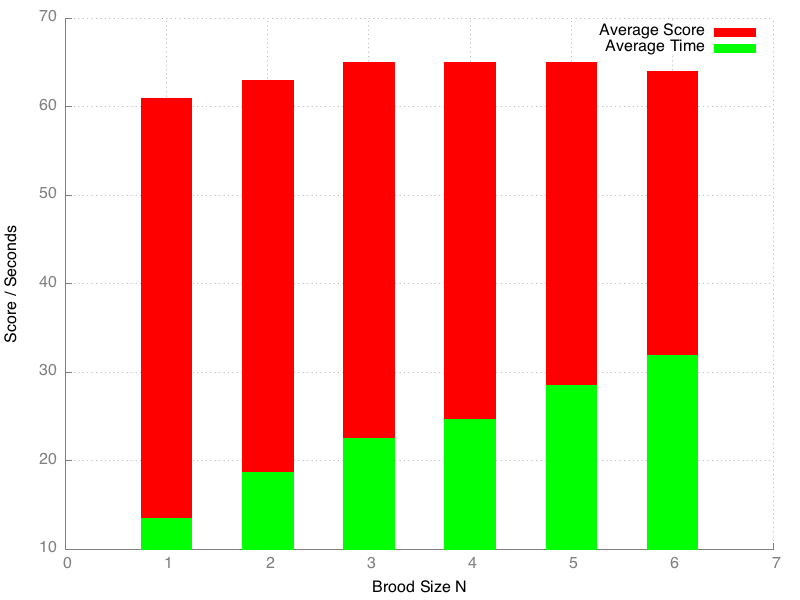
\includegraphics[width=.9\linewidth]{./results.png}
\caption{\label{fig:Figure-1}Average Score and Average Time}
\end{figure}

\begin{figure}
\centering
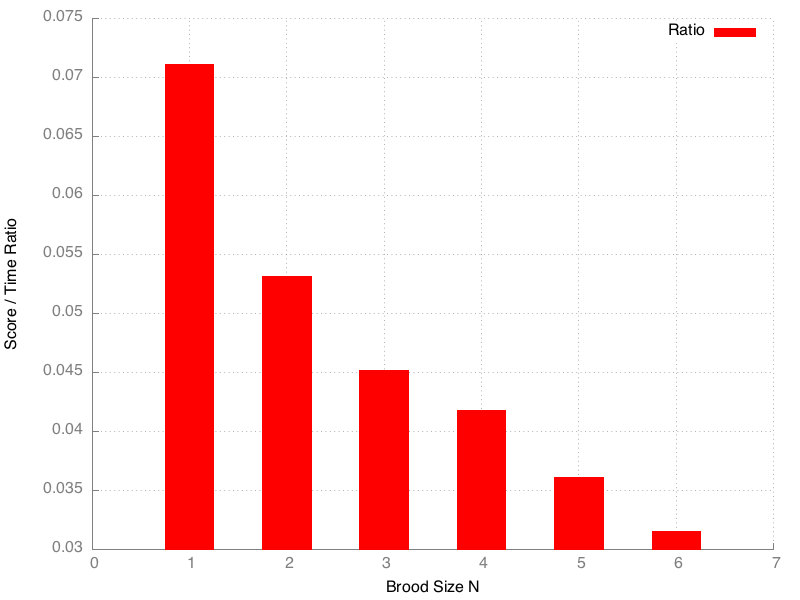
\includegraphics[width=.9\linewidth]{./results-ratios.png}
\caption{\label{fig:Figure-2}Ratio of Score / Time}
\end{figure}

%
% The following two commands are all you need in the
% initial runs of your .tex file to
% produce the bibliography for the citations in your paper.
\bibliographystyle{abbrv}
\bibliography{write-up}  % write-up.bib is the name of the Bibliography in this case
% You must have a proper ".bib" file
%  and remember to run:
% latex bibtex latex latex
% to resolve all references
%
% ACM needs 'a single self-contained file'!
%
\balancecolumns
% That's all folks!
\end{document}
